\documentclass[conference]{IEEEtran}

\usepackage[T1]{fontenc}
\usepackage[utf8]{inputenc}
\usepackage{cite}
\usepackage{amsmath,amssymb,amsfonts}
\usepackage{graphicx}
\usepackage{booktabs}
\usepackage{array}
\usepackage{multirow}
\usepackage{url}
\usepackage{microtype}
\usepackage[hidelinks]{hyperref}
\usepackage{placeins}

% Tighten float spacing to reduce large gaps around figures/tables.
\setlength{\textfloatsep}{8pt plus 1pt minus 2pt}
\setlength{\dbltextfloatsep}{8pt plus 1pt minus 2pt}
\setlength{\floatsep}{8pt plus 1pt minus 2pt}
\setlength{\intextsep}{8pt plus 1pt minus 2pt}

\newcolumntype{L}[1]{>{\raggedright\arraybackslash}p{#1}}
\setlength{\emergencystretch}{2em}

\begin{document}

\title{Understanding Structural and Behavioural Drivers of Sentiment--Rating Incongruence in Sri Lanka Tourism Reviews}

\author{}

\maketitle

\begin{abstract}
Star ratings are widely used as ground-truth sentiment labels in opinion mining, yet their alignment with review text remains under-examined. This study investigates sentiment--rating incongruence, the mismatch between star ratings and textual sentiment, using 16,156 tourism attraction reviews from Sri Lanka. A transformer-based sentiment pipeline identifies incongruence in 18.6\% of reviews, structured across six directional patterns, with Conservative Rater and Obligatory 5-Star behaviours accounting for 66.7\% of all mismatches. Incongruence varies significantly across venue types ($\chi^2 = 125.85$, $p < 0.001$), with museums exhibiting the highest rates. A multi-stage analytical framework, combining statistical tests, logit modeling, Random Forest, and SHAP, reveals venue type, reviewer expertise, and review length as key predictors. Predictive performance remains modest (AUC $\approx 0.58$--$0.61$), indicating that incongruence is structured yet only partially explainable using observable features. These findings challenge the assumption, ratings reliably represent textual sentiment and highlight the presence of systematic label distortion in review data, with implications for sentiment modeling and tourism platform design.
\end{abstract}

\begin{IEEEkeywords}
Sentiment Analysis, Sentiment-Rating Incongruence, Tourism Reviews, Sri Lanka, Logistic Regression, SHAP
\end{IEEEkeywords}

\section{Introduction}
Tourism reviews are a key source of information for travel decisions, with most platforms presenting both star ratings and written text. In sentiment analysis, these ratings are commonly treated as ground-truth labels, providing a convenient mapping to sentiment polarity \cite{ref1}, \cite{ref2}. However, this assumption remains under-examined, as ratings and text do not always align, introducing systematic noise into downstream models. The rapid growth of user-generated content on platforms such as TripAdvisor has dramatically increased the volume of available review data \cite{ref9}, yet the reliability of numerical ratings as proxies for textual sentiment has not been proportionately scrutinised.

Such divergence is not necessarily erroneous but reflects consistent reviewer behaviour shaped by expectations, experience, and context. We define this phenomenon as sentiment--rating incongruence and treat it as a structured behavioural pattern rather than a labeling issue. Evidence from large-scale review datasets suggests that over 40\% of reviews exhibit some form of inconsistency between sentiment polarity and assigned rating scores \cite{ref5}, \cite{ref6}, underscoring that the assumption of alignment is empirically fragile. Deep learning approaches, including transformer-based models, have demonstrated superior capacity to capture such nuanced divergences compared to traditional lexicon-based methods \cite{ref10}, \cite{ref11}.

Despite its importance, incongruence remains insufficiently studied. Prior work continues to rely on ratings as proxy labels, largely focusing on hotels and restaurants in well-studied regions \cite{ref2}, \cite{ref12}. Topic modelling and aspect-based sentiment analysis have extended our understanding of how specific service dimensions relate to overall ratings \cite{ref13}, \cite{ref14}, yet the broader question of systematic incongruence across review types and venue categories has received limited attention. Studies in Sri Lanka report rating--text incompatibility in hotel reviews \cite{ref3}, \cite{ref4}, while broader research highlights contextual variation and systematic inconsistency \cite{ref5,ref6,ref7}.

There is limited understanding of its prevalence, structure, and drivers, particularly for tourism attractions. Existing systematic reviews of sentiment analysis in hospitality \cite{ref12} confirm that attraction reviews in emerging destinations are substantially understudied relative to hotels and restaurants. Furthermore, the potential for zero-shot and transfer learning approaches to operate without labelled data \cite{ref15} opens new avenues for characterising incongruence at scale without manual annotation overhead. This study addresses these gaps using 16,156 Sri Lankan attraction reviews (2010--2023) \cite{ref8}, providing a systematic analysis of how sentiment is encoded differently across textual and numerical channels.

\section{Related Work}
The foundational survey by Pang and Lee \cite{ref1} established sentiment analysis as a formal discipline, embedding the assumption that star ratings reflect textual sentiment. Despite acknowledged imperfections, this convention persists in tourism research as a practical labeling strategy and baseline supervisory signal. Alaei, Becken, and Stantic \cite{ref2} observe that ratings are widely used as weak labels without explicit validation, with research heavily concentrated on hotels and restaurants. This imbalance is further confirmed by Ameur, Hamdi, and Ben Yahia \cite{ref12}, who highlight limited venue diversity and geographic coverage in existing studies, particularly for emerging tourism destinations.

Methodological advances have significantly improved sentiment analysis capabilities. Wen, Liang, and Zhu \cite{ref10} demonstrate the effectiveness of transformer-based models such as BERT and ERNIE, while Puh and Bagic Babac \cite{ref11} show that predicting both sentiment and ratings yields more granular insights. Multilingual and aspect-based approaches further enhance interpretability \cite{ref13}, \cite{ref14}, and recent zero-shot methods enable analysis in data-scarce contexts without extensive annotation \cite{ref15}.

In the Sri Lankan context, Abeysinghe and Bandara \cite{ref3}, \cite{ref4} document rating--text incompatibility in hotel reviews, but rely on lexicon-based methods and treat inconsistency primarily as a labeling issue. In contrast, this study extends the scope to tourism attraction reviews, employs transformer-based models, and frames incongruence as a behavioural phenomenon requiring explanation rather than correction, thereby shifting the analytical perspective.

Empirical evidence on rating--text alignment remains mixed. Bigne et al. \cite{ref5} report general alignment with contextual variation, while George and Ramos \cite{ref9} find ratings systematically exceed sentiment values at the destination level. Kwon et al. \cite{ref6} further demonstrate that inconsistency varies with context and influences perceived review usefulness.

Reviewer characteristics also play a critical role. Chua and Banerjee \cite{ref7} show that reviewer expertise affects the relationship between ratings and textual content, while prior work links sentiment polarity and review depth to perceived usefulness \cite{ref7}, \cite{ref12}, indicating that ratings and text encode distinct dimensions of user experience.

Overall, sentiment--rating incongruence remains insufficiently characterised in tourism attraction contexts, particularly in emerging destinations. Although transformer-based methods enable scalable and fine-grained analysis \cite{ref10}, \cite{ref11}, \cite{ref13}, and reduce annotation requirements \cite{ref15}, no prior study has systematically examined directional mismatch patterns and their structural drivers using a multi-venue, longitudinal dataset. This study addresses this gap using a large-scale Sri Lankan tourism review dataset spanning diverse attraction types and extended temporal coverage \cite{ref8}, providing new empirical evidence from an underrepresented setting.

\section{Methodology}
\subsection{Dataset and Preprocessing}

The analysis uses the “Tourism and Travel Reviews: Sri Lankan Destinations” dataset from Mendeley Data \cite{ref8}, comprising 16,156 reviews with both structured attributes and text. Sri Lanka’s diverse tourism landscape creates a heterogeneous evaluation context where rating–text inconsistencies are likely. As an underexplored emerging destination, it offers insight beyond the developed-region focus of prior work. Its scale and temporal coverage enable analysis of systematic patterns and evolving reviewer behaviour.



\begin{table}[htbp]
\caption{Dataset Attributes}
\label{tab:dataset_attributes}
\centering
\resizebox{\columnwidth}{!}{%
\begin{tabular}{L{2.8cm}L{4.2cm}L{1.8cm}}
\toprule
\textbf{Feature} & \textbf{Description} & \textbf{Data Type} \\
\midrule
Location\_Name & Name of the tourism attraction & Categorical \\
Located\_City & City where the attraction is located & Categorical \\
Location & Raw location string (may include city, district, province) & Categorical \\
Location\_Type & Category of attraction (e.g., museum, beach, temple) & Categorical \\
User\_ID & Unique identifier for the reviewer & Categorical \\
User\_Location & Free-text location of the reviewer & Categorical \\
User\_Locale & Locale/language setting (e.g., en\_US) & Categorical \\
User\_Contributions & Number of contributions made by the reviewer & Numerical \\
Travel\_Date & Date of visit & Categorical \\
Published\_Date & Date when the review was posted & Categorical \\
Rating & Numerical rating (1--5 stars) & Categorical \\
Helpful\_Votes & Number of users who found the review helpful & Numerical \\
Title & Short title of the review & Categorical \\
Text & Full review content & Categorical \\
\bottomrule
\end{tabular}%
}
\end{table}

The preprocessing pipeline includes data inspection, missing value handling, and duplicate removal. Temporal features are extracted from \textit{Travel\_Date} and \textit{Published\_Date}, including \textit{Travel\_Year} and \textit{Publication\_Year}, and \textit{Review\_Delay\_Days} is derived to capture the time gap between visit and review (with negative values corrected). Spatial information is standardized via rule-based normalization, extracting \textit{Province} and \textit{District} from \textit{Travel\_Location}, while \textit{User\_Country} is inferred from \textit{User\_Location} using text normalization and dictionary matching. Additional features include \textit{Review\_Length} and \textit{Rating\_Class}, which maps ratings into Positive (4--5), Neutral (3), and Negative (1--2) categories following standard practice \cite{ref1}, \cite{ref2}. Redundant attributes are removed, producing a dataset ready for analysis and modeling. 

\subsection{Sentiment Model Selection for Prediction}
To generate sentiment labels for the full corpus ($n = 16{,}156$), multiple candidate models were evaluated using a manually annotated subset of 1,000 reviews labeled as Positive, Neutral, or Negative based on combined title and text interpretation. The data were stratified into 700 training and 300 test samples. Two models (Cardiff RoBERTa and RoBERTa-base) were fine-tuned on the training set, while all pretrained and fine-tuned models were evaluated on the same held-out test set under a consistent pipeline. Titles and text were concatenated, and long inputs were handled using a sliding-window chunking strategy, with predictions aggregated via probability averaging to obtain review-level sentiment.Performance was evaluated using Macro F1 (primary, due to class imbalance), along with Accuracy and Weighted F1. The pretrained \textit{cardiffnlp/twitter-roberta-base-sentiment} model was selected for corpus-wide prediction, as it provided the best overall balance (Accuracy = 0.8300, Weighted F1 = 0.8051, Macro F1 = 0.6918), despite the fine-tuned RoBERTa-base achieving the highest Macro F1 (0.6984). The pretrained model also improves reproducibility by avoiding task-specific fine-tuning.


 
\begin{table*}[t]
\caption{Sentiment Model Performance on Test Set ($n = 300$)}
\label{tab:sentiment_performance}
\centering
\resizebox{\textwidth}{!}{%
\begin{tabular}{L{6.0cm}cccccL{4.3cm}}
\toprule
\textbf{Candidate Model} & \textbf{Accuracy} & \textbf{Macro Precision} & \textbf{Macro Recall} & \textbf{Macro F1} & \textbf{Weighted F1} & \textbf{Selection Note} \\
\midrule
gosorio/robertaSentimentFT\_TripAdvisor & 0.7300 & 0.2433 & 0.3333 & 0.2813 & 0.6161 & Rejected (poor minority-class performance) \\
cardiffnlp/twitter-roberta-base-sentiment (pretrained) & 0.8300 & 0.7420 & 0.6889 & 0.6918 & 0.8051 & Selected for corpus-wide prediction \\
Fine-tuned Cardiff RoBERTa (700/300, chunked) & 0.7333 & 0.6531 & 0.7377 & 0.6768 & 0.7576 & Strong recall, lower overall stability \\
Fine-tuned roberta-base (700/300, chunked) & 0.7767 & 0.6781 & 0.7234 & 0.6984 & 0.7801 & Highest Macro F1, slightly lower overall balance \\
\bottomrule
\end{tabular}%
}
\end{table*}

\subsection{Sentiment Prediction and Analytical Variables}
Using the selected sentiment model, a new categorical variable, \textit{Sentiment}, was generated for all reviews in the dataset. This variable represents the predicted polarity of each review based on the combined textual content of the title and review body. Afterwards \textit{Title} and \textit{Text} columns were removed. To support subsequent statistical analysis, three core analytical variables were derived without additional predictive modeling:

\begin{itemize}
\item \textbf{Incongruent:} Incongruence (0/1) was defined by comparing \textit{Rating\_Class} and \textit{Sentiment}, with matching polarity treated as congruent and all other combinations as incongruent.
\item \textbf{Pattern:} A six-category variable captures directional mismatches beyond binary incongruence.
\item \textbf{Reviewer\_Tier:} \textit{Reviewer\_Tier} was derived from \textit{User\_Contributions} as an ordinal variable to capture reviewer activity. Given the highly right-skewed distribution (mean = 191.6, median = 54, max = 9010), contributions were grouped into four tiers: Novice (0--5), Casual (6--20), Active (21--100), and Expert (101+). These thresholds reflect the empirical distribution, distinguishing infrequent from highly active contributors while preserving the long-tailed participation structure. The resulting distribution (Active: 37.2\%, Expert: 35.0\%, Casual: 19.7\%, Novice: 8.0\%) provides balanced representation for statistical analysis. Continuous variables (\textit{Review\_Length}, \textit{Review\_Delay\_Days}) were log-transformed using $\log(1 + x)$ to reduce skewness. All variables were deterministically derived to ensure reproducibility, and \textit{User\_Contributions} was removed after feature construction. \end{itemize} 

\subsection{Statistical Procedures and Model Validation}
The final phase integrates statistical testing, predictive modeling, and model interpretation to validate the analytical framework and identify key drivers of sentiment--rating incongruence. \textit{Location\_Name and Located\_City} were excluded due to high cardinality and redundancy with higher-level spatial features (\textit{Province, Location\_Type}). \textit{User\_Country} and \textit{User\_Locale} were omitted due to sparsity and inconsistent formatting, limiting their reliability for statistical testing. \textit{Published\_Date, Travel\_Date} and \textit{Published\_Year} were not directly modeled as its information is captured through derived temporal variables (\textit{Travel\_Year, Review\_Delay}), while \textit{Title\_Length} was excluded due to its high correlation with \textit{Review\_Length}, to avoid redundancy and multicollinearity. Temporal variables were modeled using a centered linear term (\textit{Travel\_Year\_c}) and a quadratic term (\textit{Travel\_Year\_c$^2$}), obtained by mean-centering the travel year and squaring it. Centering reduces multicollinearity between polynomial terms, while the quadratic term tests for nonlinear temporal trends in incongruence. 

\subsubsection{Exploratory and Association Testing}
Incongruence prevalence is computed as a proportion of total reviews. Associations with categorical variables (Location\_Type, Reviewer\_Tier, Province) are evaluated using Chi-square tests with effect sizes reported via Cramér’s V. For Location\_Type, odds ratios (OR) are computed relative to National Parks (reference), where odds are defined as the ratio of incongruent to congruent reviews. National Parks are selected due to their lowest incongruence rate and relatively uniform evaluation context, providing a stable baseline for comparison with more heterogeneous venue types (e.g., museums, religious sites). For continuous variables (Review\_Length, Review\_Delay, Travel\_Year), group differences are assessed using the Mann–Whitney U test due to non-normality. To control for multiple comparisons, p-values are adjusted using the Benjamini–Hochberg False Discovery Rate (FDR) procedure with a significance threshold of q < 0.05.

 

\subsubsection{Predictive Modeling Framework}
The target variable for all predictive models is the binary \textit{Incongruent} flag (0 = congruent, 1 = incongruent), as the objective is to explain the factors driving sentiment--rating mismatch rather than predict sentiment itself. Variables used to construct this target (\textit{Sentiment, Rating, Rating\_Class}) were excluded to prevent data leakage. The predictor set comprises 24 features capturing structural, behavioural, temporal, and textual characteristics: \textit{Location\_Type} (\textit{LT\_Museums, LT\_Beaches, LT\_Bodies of Water, LT\_Religious Sites, LT\_Zoological Gardens, LT\_Waterfalls, LT\_Nature \& Wildlife Areas, LT\_Gardens, LT\_Farms, LT\_Historic Sites}), province (\textit{PV\_Northern Province, PV\_North Central Province, PV\_Central Province, PV\_Uva Province, PV\_Western Province, PV\_Sabaragamuwa Province, PV\_Eastern Province}), \textit{Reviewer\_Tier} (\textit{Tier\_Casual, Tier\_Active, Tier\_Expert}), temporal variables (\textit{Travel\_Year\_c, Travel\_Year\_c$^2$}), and review characteristics (\textit{log\_review\_length, log\_review\_delay}). Categorical variables were dummy encoded with National Parks, Southern Province, and Novice reviewers as reference categories, while continuous variables were log-transformed and temporal variables centered to address skewness and capture nonlinear trends. Although all categories are included in statistical tests, one category is omitted during model estimation to avoid multicollinearity, enabling interpretation relative to a baseline without loss of information.

The analytical framework integrates statistical testing, modeling, and interpretation in a structured pipeline. Bivariate tests (Chi-square and Mann--Whitney U), with FDR correction, identify variables associated with incongruence but do not account for confounding; thus, resulting odds ratios represent unadjusted effects. A statsmodels logit model (Model 1B) addresses this by estimating independent effects through adjusted odds ratios and confidence intervals, while logistic regression (Model 1A) provides a baseline measure of linear predictive performance. AUC-ROC is used as the primary evaluation metric due to its robustness to class imbalance and threshold independence. To capture nonlinearities and interactions beyond the linear framework, a Random Forest model (Model 2) is employed, with SHAP used for interpretation. SHAP quantifies feature importance and reveals context-dependent effects. The pipeline progresses from association (statistical tests) to explanation (logit model) to behavioural interpretation (Random Forest + SHAP): statistical tests identify relationships, the logit model isolates independent effects, and the Random Forest captures nonlinear patterns, with SHAP translating these into interpretable feature contributions. Together, this integrated approach combines statistical rigor and data-driven modeling to characterize incongruence as a structured yet partially latent phenomenon.

 

\section{Results}
\subsection{Prevalence and Six-Pattern Typology}
Of the 16,156 tourism attraction reviews analyzed, 3,005 are identified as incongruent, yielding an overall prevalence of 18.6\%, or approximately one in five reviews.

\begin{table}[htbp]
\caption{Six Directional Incongruence Patterns ($n = 3{,}005$ incongruent reviews)}
\label{tab:six_patterns}
\centering
\resizebox{\columnwidth}{!}{%
\begin{tabular}{cL{3.0cm}L{2.5cm}L{2.2cm}cL{4.3cm}}
\toprule
\# & Pattern & Rating & Sentiment & $n$ & \% of Incongruent / \% of All \\
\midrule
1 & Conservative Rater & Neutral (3$\star$) & POSITIVE & 1,155 & 38.4\% / 7.1\% \\
2 & Obligatory 5-Star & Positive (4--5$\star$) & NEUTRAL & 851 & 28.3\% / 5.3\% \\
3 & Frustrated Neutral & Neutral (3$\star$) & NEGATIVE & 509 & 16.9\% / 3.2\% \\
4 & Polite Inflator & Positive (4--5$\star$) & NEGATIVE & 219 & 7.3\% / 1.4\% \\
5 & Harsh Deflator & Negative (1--2$\star$) & NEUTRAL & 160 & 5.3\% / 1.0\% \\
6 & Punitive Rater & Negative (1--2$\star$) & POSITIVE & 111 & 3.7\% / 0.7\% \\
\bottomrule
\end{tabular}%
}
\end{table}
Incongruence is further characterized using a six-pattern typology (Table~\ref{tab:six_patterns}). The Conservative Rater (38.4\%) and Obligatory 5-Star (28.3\%) patterns together account for 66.7\% of incongruent reviews, indicating that mismatch is directionally structured rather than random. Patterns such as Frustrated Neutral and Polite Inflator (24.2\% combined) reflect negative sentiment paired with non-negative ratings, consistent with face-saving behaviour. These structured patterns motivate further analysis across contextual and reviewer-related factors. 

\subsection{Variation Across Venue Types}
To examine contextual variation, incongruence rates were compared across 11 attraction categories. A chi-square test confirms a statistically significant association between venue type and incongruence ($\chi^2(10) = 125.85$, $p < 0.001$), with a small but meaningful effect size (Cramer's V = 0.088).

A clear gradient is observed (Table~\ref{tab:venue_type_rates}), with National Parks exhibiting the lowest incongruence rate (12.8\%) and Museums the highest (26.3\%). This corresponds to an odds ratio of 2.43, indicating that museum reviews are more than twice as likely to be incongruent relative to the baseline. The 13.5 percentage-point spread across categories is both substantial and systematically structured, suggesting that mismatch varies meaningfully with contextual characteristics of the experience.

\begin{table}[htbp]
\caption{Incongruence Rate by Venue Type, Ranked (Reference: National Parks)}
\label{tab:venue_type_rates}
\centering
\resizebox{\columnwidth}{!}{%
\begin{tabular}{L{3.0cm}cc}
\toprule
Venue Type & Incongruence Rate & OR vs. National Parks \\
\midrule
Museums & 26.3\% & 2.43 \\
Beaches & 19.0\% & 1.60 \\
Religious Sites & 19.8\% & 1.68 \\
Bodies of Water & 23.7\% & 2.12 \\
Gardens & 17.4\% & 1.43 \\
Farms & 16.6\% & 1.35 \\
Waterfalls & 18.0\% & 1.50 \\
Nature \& Wildlife Areas & 16.4\% & 1.34 \\
Zoological Gardens & 21.6\% & 1.88 \\
Historic Sites & 15.6\% & 1.26 \\
National Parks & 12.8\% & 1.00 (ref) \\
\bottomrule
\end{tabular}%
}
\end{table}

These findings indicate that incongruence is not uniformly distributed, motivating a more formal examination of potential predictors.

\subsection{Predictors of Incongruence}
\textbf{Bivariate screening with FDR correction.} Initial statistical screening was conducted to identify variables associated with incongruence at the bivariate level. As shown in Table~\ref{tab:bivariate_screening}, four of five predictors remain significant after Benjamini--Hochberg FDR correction. Reviewer tier, province, travel year, and review length all show significant associations, while review delay is non-significant ($q = 0.7503$), providing no evidence that the timing between visit and review influences mismatch.

\begin{table}[htbp]
\caption{Bivariate Predictor Screening with Benjamini--Hochberg FDR Correction}
\label{tab:bivariate_screening}
\centering
\resizebox{\columnwidth}{!}{%
\begin{tabular}{L{2.0cm}L{1.8cm}L{1.3cm}L{1.3cm}L{1.0cm}}
\toprule
Predictor & Test Statistic & Raw $p$ & $q$-value & Retained \\
\midrule
Reviewer Tier & $\chi^2(3)=85.99$ & $1.59\times10^{-18}$ & $7.94\times10^{-18}$ & Yes \\
Province & $\chi^2(7)=49.10$ & $2.17\times10^{-8}$ & $3.62\times10^{-8}$ & Yes \\
Travel Year & Mann--Whitney & $7.73\times10^{-11}$ & $1.93\times10^{-10}$ & Yes \\
Review Length & Mann--Whitney & 0.0011 & 0.0014 & Yes \\
Review Delay & Mann--Whitney & 0.7503 & 0.7503 & No \\
\bottomrule
\end{tabular}%
}
\end{table}

\textbf{Incongruence Across Reviewer Tiers.} At the bivariate level, expert reviewers are 1.97 times more likely than novices to produce incongruent reviews, and incongruent reviews are longer at the median (296 vs. 279 characters), suggesting that verbosity increases the likelihood of divergence between text and rating. While these results establish meaningful associations, they do not account for confounding effects between variables. Therefore, multivariate modeling is required to identify independent predictors.

\textbf{Multicollinearity check.}VIF analysis shows no multicollinearity (max = 3.663, mean = 2.186)

\subsection{Model-Based Analysis and Interpretation}
\subsubsection{Model 1A -- Logistic Regression (Baseline Discrimination)}
A class-balanced logistic regression model with five-fold stratified cross-validation achieves a mean CV AUC of  $0.5890 \pm 0.0093$  and a test AUC of 0.5840, indicating modest but stable performance. This baseline captures the linear predictive signal, while the low AUC suggests that incongruence is influenced by latent behavioural factors beyond observable features. 


\subsubsection{Model 1B -- Explanatory Logit (Primary Inference Model)}
A statsmodels logit model was fitted to identify independent predictors of incongruence, with adjusted odds ratios accounting for all other variables. Statistical significance was assessed using 95\% confidence intervals (CI), where predictors are significant if the CI excludes 1. A total of 19 predictors meet this criterion, indicating strong systematic relationships. 

Venue type emerges as a key determinant. Relative to National Parks, Museums (OR = 2.386), Beaches (2.171), Bodies of Water (2.022), Religious Sites (1.492), Zoological Gardens (1.725), Waterfalls (1.324), and Nature \& Wildlife Areas (1.279) show significantly higher odds of incongruence (CI $>$ 1). In contrast, Gardens (1.265), Farms (1.224), and Historic Sites (1.163) are not statistically significant (CI includes 1), indicating no clear effect.

Reviewer expertise exhibits a clear gradient, with Expert (1.740), Active (1.522), and Casual (1.243) reviewers all significantly more likely to produce incongruence compared to Novices, consistent with a calibration-based interpretation of rating behaviour.

Geographic effects are also evident. Several provinces show elevated odds, including Northern (1.787), Sabaragamuwa (1.641), North Central (1.601), Central (1.586), Uva (1.523), and Western (1.382), while Eastern Province (1.066) is not significant.

Review characteristics indicate that review length (OR = 1.219) has a strong positive association with incongruence, whereas review delay (OR = 0.960) shows a weak but statistically significant negative effect, suggesting only a marginal influence.

Temporal effects reveal a significant negative association for Travel\_Year\_c (OR = 0.946, CI $<$ 1), indicating that incongruence decreases over time. The quadratic term (Travel\_Year\_c$^2$: OR = 0.995) is not statistically significant, providing no evidence of nonlinear temporal effects and suggesting an approximately linear trend.

Overall, the model provides the study's primary explanatory insight by quantifying the independent and directional effects of structural, behavioural, temporal, and contextual predictors on the likelihood of incongruence.

\subsubsection{Model 2 -- Random Forest (Nonlinear Structure Assessment)}
To capture nonlinear relationships and interactions, a Random Forest model was trained on the same dataset. It achieves a test AUC of 0.6095, improving by +0.0256 over logistic regression, confirming the presence of nonlinear effects. However, the modest gain indicates these effects are not dominant, positioning the Random Forest as a complementary diagnostic model rather than a replacement for the logit.

\subsubsection{SHAP Analysis -- Interpreting Nonlinear Behaviour}
SHAP analysis was applied to the Random Forest to interpret feature effects. Mean absolute SHAP values identify review length (0.0306), expert tier (0.0273), Travel\_Year\_c (0.0219), review delay (0.0203), and museums (0.0182) as the most influential predictors.The SHAP summary shows that longer reviews increase incongruence, expert reviewers contribute positively (less experienced negatively), and incongruence declines over time—consistent with the logit model. Review delay has a modest, context-dependent effect, aligning with its non-significance in bivariate analysis and weak logit impact, suggesting interaction-driven influence. SHAP complements the logit by revealing nonlinear, context-dependent effects. 

 

\begin{figure}[htbp]
\centering
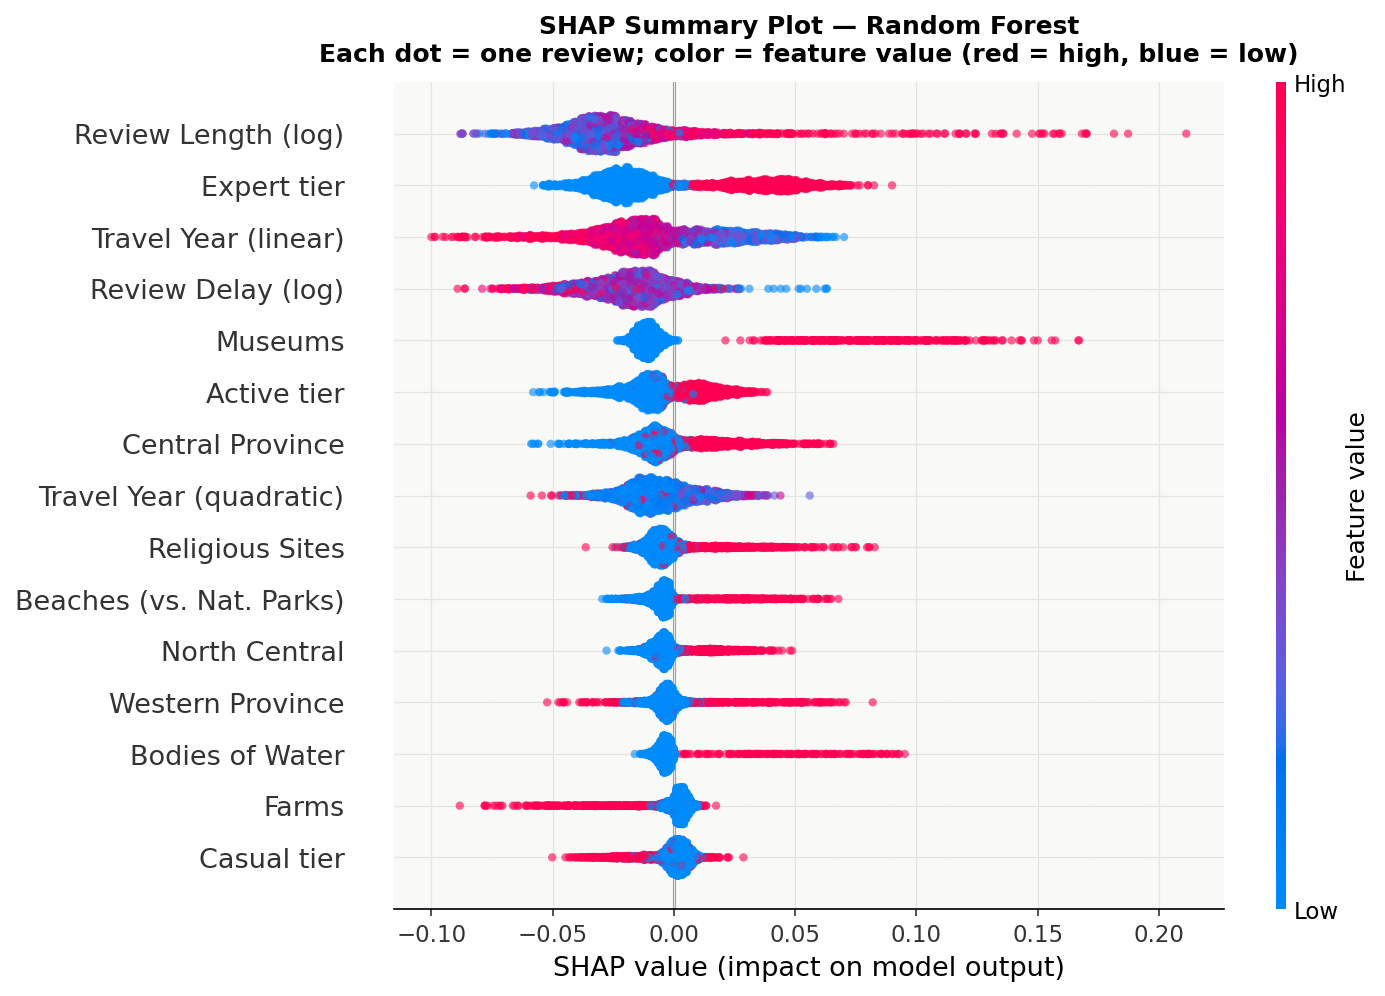
\includegraphics[width=\columnwidth]{fig7b_shap_summary.png}
\caption{SHAP summary plot for the Random Forest model.}
\label{fig:shap_summary}
\end{figure}

\section{Discussion}
\subsection{Structured Incongruence and Conservative Rating Behaviour }
An incongruence rate of 18.6\% (\~1 in 5 reviews) indicates systematic mismatch rather than random noise. In Sri Lanka, religious sites may induce high ratings despite mixed sentiment, while museums require multidimensional evaluation not captured by a single score; experienced reviewers may also write positively but rate conservatively. This structured, context-dependent behaviour is further reflected in the Conservative Rater pattern—positive text with moderate ratings—which accounts for 38.4\% of incongruent reviews and represents the dominant mechanism of mismatch. Its prevalence increases from 27.4\% (novice) to 40.4\% (expert), supporting a calibration effect where experienced reviewers apply stricter standards. Together, these findings show that incongruence is systematic rather than random. \textbf{Implication:} Star ratings are unreliable ground-truth labels, and models may misinterpret positive experiences as neutral—particularly for expert-generated content—leading to systematic bias.


\subsection{Location Type as a Structural Moderator of Label Reliability}
Location type is a key determinant of incongruence. Museum reviews show higher odds of mismatch (Adjusted OR = 2.386) relative to national parks, with similar effects for beaches and bodies of water; zoological gardens and waterfalls are also significant. This reflects evaluative complexity, as multidimensional experiences (e.g., museums) are harder to capture with a single rating, while religious sites may show higher mismatch due to social pressures. These results indicate that label reliability varies with context. \textbf{Implication:} Treating all reviews uniformly may introduce systematic bias, highlighting the need for context-aware sentiment models. 

\subsection{Complementary Roles of Linear and Nonlinear Models}
The multi-model framework demonstrates that linear and nonlinear approaches provide complementary layers of insight rather than competing explanations. The logistic regression baseline achieves a test AUC of 0.584, establishing a stable reference for linear discriminative capacity, while the explanatory logit model identifies 19 statistically significant predictors, providing interpretable effect sizes and clear directional relationships. The Random Forest model achieves a higher test AUC of 0.6095, confirming the presence of nonlinear relationships and interaction effects. However, the modest gain indicates nonlinearities are secondary drivers of incongruence. 

Importantly, the overall predictive performance (AUC $\approx 0.58$--$0.61$) should not be viewed as a limitation of model quality, but as evidence of the inherently complex and partially unobservable nature of the phenomenon. While statistically significant predictors exist, their moderate effect sizes suggest that the signal is distributed across multiple factors, with remaining variation driven by latent behavioural processes such as reviewer calibration and contextual norms. This establishes a key contribution: modest predictive performance itself is an informative finding, demonstrating that incongruence is structured yet difficult to predict. SHAP analysis reinforces this interpretation by revealing how features such as reviewer expertise, review length, and venue type contribute in nonlinear and context-dependent ways. Crucially, these insights do not contradict the logit model; instead, they show that nonlinear methods capture heterogeneity within effects that linear models necessarily average. This implies that improving predictive performance requires incorporating latent behavioural and contextual signals, and that star ratings are not fully reliable ground-truth labels due to systematic, context-dependent distortions. 

\subsection{Review Delay and Reviewer Expertise Effects }
Review delay shows no significant effect in bivariate analysis and only a weak negative association in the logit model (OR = 0.960). Although ranked as relatively influential by SHAP, its effect is modest and context-dependent, indicating it is a secondary factor rather than a primary driver of incongruence. In contrast, mismatch patterns vary systematically with reviewer expertise: Conservative Rater behaviour increases from 27.4\% (novice) to 40.4\% (expert), while extreme patterns such as Harsh Deflator decrease from 10.8\% to 4.2\%.This suggests experienced reviewers are more calibrated, with incongruence driven more by reviewer traits than time, underscoring the need for reviewer-level modelling.

 


\section{Conclusion}
This study shows that sentiment–rating incongruence in tourism reviews is not random noise but a structured phenomenon driven by reviewer behaviour and contextual evaluation complexity. Using statistical inference, predictive modelling, and interpretable machine learning, mismatch is linked to mechanisms such as reviewer calibration, multidimensional evaluation, and context-specific rating norms. Several limitations should be noted. The analysis is based on a single Sri Lankan dataset, limiting generalizability. It relies on structured features and sentiment labels, which may introduce measurement error and overlook deeper linguistic nuances. The modest predictive performance (AUC $\approx$ 0.58–0.61) suggests substantial unexplained variance, likely driven by latent behavioural and contextual factors, and the observational design limits causal inference. Despite this, the findings highlight a key insight: incongruence is structured yet only partially observable, revealing limitations in treating star ratings as reliable ground truth. This has important implications for NLP and platform design, as systematic label distortion may bias models and aggregated ratings may underrepresent true sentiment.Rating–text inconsistency is a meaningful behavioural signal, not noise; future work should extend this across contexts and incorporate deeper semantic features to improve explanatory power.

 

 

\begin{thebibliography}{15}

\bibitem{ref1}
B. Pang and L. Lee, ``Opinion mining and sentiment analysis,'' \textit{Foundations and Trends in Information Retrieval}, vol. 2, no. 1--2, pp. 1--135, 2008.

\bibitem{ref2}
A. R. Alaei, S. Becken, and B. Stantic, ``Sentiment analysis in tourism: Capitalising on big data,'' \textit{Journal of Travel Research}, vol. 58, no. 2, pp. 175--191, 2019.

\bibitem{ref3}
P. Abeysinghe and T. Bandara, ``A novel self-learning approach to overcome incompatibility on TripAdvisor reviews,'' \textit{Data Science and Management}, vol. 5, pp. 1--10, 2022.

\bibitem{ref4}
H. P. P. M. Abeysinghe and C. K. Walgampaya, ``Sentiment analysis in user reviews: A study of incompatibility in hotel reviews in city of Anuradhapura, Sri Lanka,'' in \textit{Proc. iPURSE 2021}, Peradeniya, Sri Lanka, Nov. 2021, vol. 23.

\bibitem{ref5}
E. Bigne, C. Ruiz, C. Perez-Cabanero, and A. Cuenca, ``Are customer star ratings and sentiments aligned? A deep learning study of the customer service experience in tourism destinations,'' \textit{Service Business}, vol. 17, pp. 281--314, 2023.

\bibitem{ref6}
B. Kwon, J. Lee, J. Min, C. Kwak, and H. B. S. Choi, ``Beyond the stars: The impact of rating-text inconsistency on perceived review usefulness,'' \textit{Asia Pacific Journal of Information Systems}, vol. 35, no. 1, pp. 49--72, 2025.

\bibitem{ref7}
A. Y. K. Chua and S. Banerjee, ``Understanding review helpfulness as a function of reviewer reputation, review rating, and review depth,'' \textit{Journal of the Association for Information Science and Technology}, vol. 66, no. 2, pp. 354--362, 2015.

\bibitem{ref8}
T. Sewwandi, ``Tourism and Travel Reviews: Sri Lankan Destinations,'' Mendeley Data, V1, 2023, doi: 10.17632/2nbvx5m4hs.1.

\bibitem{ref9}
O. A. George and C. M. Q. Ramos, ``Sentiment analysis applied to tourism: exploring tourist-generated content in the case of a wellness tourism destination,'' \textit{International Journal of Spa and Wellness}, vol. 7, no. 2, pp. 139--161, 2024.

\bibitem{ref10}
Y. Wen, Y. Liang, and X. Zhu, ``Sentiment analysis of hotel online reviews using the BERT model and ERNIE model---Data from China,'' \textit{PLOS ONE}, vol. 18, no. 3, e0275382, Mar. 2023.

\bibitem{ref11}
K. Puh and M. Bagic Babac, ``Predicting sentiment and rating of tourist reviews using machine learning,'' \textit{Journal of Hospitality and Tourism Insights}, vol. 6, no. 3, pp. 1188--1204, 2023.

\bibitem{ref12}
A. Ameur, S. Hamdi, and S. Ben Yahia, ``Sentiment analysis for hotel reviews: A systematic literature review,'' \textit{ACM Computing Surveys}, vol. 56, no. 2, Article 51, Sep. 2023.

\bibitem{ref13}
M. Chu, Y. Chen, L. Yang, and J. Wang, ``Language interpretation in travel guidance platform: Text mining and sentiment analysis of TripAdvisor reviews,'' \textit{Frontiers in Psychology}, Oct. 2022.

\bibitem{ref14}
T. Ali, B. Omar, and K. Soulaimane, ``Analyzing tourism reviews using an LDA topic-based sentiment analysis approach,'' \textit{MethodsX}, vol. 9, 101894, Nov. 2022.

\bibitem{ref15}
I. Nawawi, K. F. Ilmawan, M. R. Maarif, and M. Syafrudin, ``Exploring tourist experience through online reviews using aspect-based sentiment analysis with zero-shot learning for hospitality service enhancement,'' \textit{Information}, vol. 15, no. 8, p. 499, Aug. 2024.

\end{thebibliography}

\end{document}
